%% General definitions
\documentclass{article} %% Determines the general format.
\usepackage{a4wide} %% paper size: A4.
\usepackage[utf8]{inputenc} %% This file is written in UTF-8.
%% Some editors on Windows cannot save files in UTF-8.
%% If there is a problem with special characters not showing up
%% correctly, try switching "utf8" to "latin1" (ISO 8859-1).
\usepackage[T1]{fontenc} %% Format of the resulting PDF file.
\usepackage{fancyhdr} %% Package to create a header on each page.
\usepackage{lastpage} %% Used for "Page X of Y" in the header.
                      %% For this to work, you have to call pdflatex twice.
\usepackage{enumerate} %% Used to change the style of enumerations (see below).

\usepackage{amssymb} %% Definitions for math symbols.
\usepackage{amsmath} %% Definitions for math symbols.

\usepackage{tikz}  %% Pagacke to create graphics (graphs, automata, etc.)
\usetikzlibrary{automata} %% Tikz library to draw automata
\usetikzlibrary{arrows}   %% Tikz library for nicer arrow heads
\usetikzlibrary{positioning}    %% Tikz library for more positioning options

\usepackage{hyperref} %% hyperlinks

%% Left side of header
\lhead{\course\\\semester\\Exercise \homeworkNumber}
%% Right side of header
\rhead{\authorname\\Page \thepage\ of \pageref{LastPage}}
%% Height of header
\usepackage[headheight=36pt]{geometry}
%% Page style that uses the header
\pagestyle{fancy}

\newcommand{\authorname}{Benjamin Regez\\Luis Tritschler}
\newcommand{\semester}{Spring Semester 2026}
\newcommand{\course}{Foundations of Artificial Intelligence}
\newcommand{\homeworkNumber}{4}

\renewcommand{\thesection}{Exercise \homeworkNumber.\arabic{section}}


\begin{document}

\section{Iterative Deepening DFS}
\begin{enumerate}[(a)]
    \item See file \texttt{IterativeDeepeningSearch.java}.
    
    \item Metrics of Pancake instances run with implementation:\\
    \begin{table}[h!]
    \begin{tabular}{rrrrrr}
    \hline
    \\[-0.8em]
     & & & \multicolumn{2}{c}{generated nodes} & \\[0.2em] \cline{4-5} \\[-0.8em]
    instance & result & runtime & last iteration & total & solution length  \\[0.2em] \hline
    \\[-0.8em]
    01 & solved & 0.008 & 5 429 & 7 294 & 5 \\[0.2em] \hline
    \\[-0.8em]
    02 & solved & 0.0179 & 27 188 & 50 063 & 6 \\[0.2em] \hline
    \\[-0.8em]
    03 & solved & 0.0163 & 34 722 & 40 071 & 5 \\[0.2em] \hline
    \\[-0.8em]
    04 & solved & 0.0568 & 320 633 & 395 366 & 6 \\[0.2em] \hline
    \\[-0.8em]
    05 & solved & 23.75 & 353 307 323 & 476 764 112 & 9 \\[0.2em] \hline
    \\[-0.8em]
    06 & solved & 76.57 & 1 325 430 609 & 1 584 804 854 & 9 \\[0.2em] \hline
    \\[-0.8em]
    07 & timeout & & > 1 333 883 997 & > 1 845 597 750 & > 9 \\[0.2em] \hline
    \\[-0.8em]
    08 & timeout & & > 883 708 281 & > 957 350 637 & > 8 \\[0.2em] \hline
    \\[-0.8em]
    09 & timeout & & > 1 589 311 291 & > 1 711 566 005 & > 8 \\[0.2em] \hline
    \\[-0.8em]
    10 & timeout & & > 2 745 954 241 & > 2 942 093 829 & > 8 \\[0.2em] \hline
    \end{tabular}
    \end{table}\\[-0.5em]
    Remark: With "solution length" we mean number of steps to the solution. E.g. length 0 means the
    initial state node is also the goal state node. \\[0.5em]
    \textcolor{red}{\textbf{Reminder for ourselves}}: \texttt{'ulimit -St 600'} must be
    entered again if wsl has been restarted.

    \item \textit{Problems 01 and 03 have the same solution lengths and therefore find solutions in the same
    iteration of iterative deepening search. Yet, they generate significantly different numbers of
    nodes before finding that solution. How is this possible given that both solve instances of
    the pancake problem?}\\[0.5em]
    Problem instance 1 has only 6 nodes: $\langle 4, 6, 1, 5, 3, 2 \rangle$,
    but instance 3 has 8 nodes: $\langle 8, 7, 4, 3, 1, 5, 6, 2 \rangle$.
    Thus, the corresponding state spaces also have 6 respectively 8 states.
    That is, the number of generated nodes grow faster in problem 3 than
    in problem 1. Although both problems have the same solution length, yet
    the DFS algorithm generates more nodes in problem 3 for each layer.
    
    \item \textit{Does your experiment from part (b) confirm the
    theoretical claim that the total number of generated nodes
    is dominated by the last iteration? Justify your answer.}\\[0.5em]
    We can observe that indeed the number of generated nodes
    is dominated by the last iteration. Instance 04 has the smallest
    ratio out of instances 01 - 05 and yet more than 0.66 of all
    nodes were generated in the last iteration (i.e., all other
    solved instances had an even larger ratio).
\end{enumerate}

\section{}
\begin{equation*}
    h(s) = \sum_{i=1}^{n-1} (|p_i - p_{i+1}| - 1)
\end{equation*}
\textit{Which of the four properties safe, goal-aware, admissible
and consistent does h satisfy?}
\begin{enumerate}[(i)]
    \item $h$ is safe, because every state in the state space can
    reach the goal state. Thus, $h^*(s) = \infty$ for all $s \in S$ with
    $h(s) = \infty$ holds. (We do not allow missing or double pancakes)

    \item $h$ is goal-aware. We will show this by direct proof:\\[0.5em]
    Let $s_1 = \langle 1, 2, ..., n-1, n \rangle$
    (i.e., $s_1$ is goal state). Thus,
    \begin{equation*}
        h(s_1) = \sum_{i=1}^{n-1} \underbrace{(\underbrace{|p_i - p_{i+1}|}_{= 1} - 1)}_{= 0}
        = 0
    \end{equation*}
    Since $s_1$ is the only goal state, we have shown that for all
    goal states the heuristic is zero.

    \item $h$ is \textbf{not} admissible. We will show this by direct proof: \\[0.5em]
    Let $s_b = \langle 3, 2, 1, 4 \rangle$. Then, $h(s_b) = 0 + 0 + 3 = 3 $.
    But since $s_b$ only needs one action to reach the goal state, namely
    \texttt{flip-3} (i.e., flip the first 3 pancakes), we have would expect
    $h^*(s_b) = 1$. Thus, $h(s_b) \not\le h^*(s_b) $.

    \item $h$ is \textbf{not} consistent. We will use the same state $s_b = \langle 3, 2, 1, 4 \rangle$
    as in (iii) with $h(s_b) = 3$ to show this statement. Let $a_3 = $ \texttt{flip-3} with
    cost($a_3$) = 1 (according to the definition of $\mathcal{S}$). Then, $s_b \xrightarrow{a_3} s_G$
    with $s_G = \langle 1, 2, 3, 4 \rangle$ and since $s_G$ is the goal state, $h(s_G) = 0$.
    We observe that $h(s) \le \text{cost}(a) + h(s')$ for all transitions $s \xrightarrow{a} s'$
    does not hold, because $3 \not\le 1 + 0$.

\end{enumerate}

\newpage
\section{}
\textit{For the state space depicted below with uniform action costs of 1, define a heuristic that is
consistent, not safe and has a perfect estimate for s0 (i.e., $h(s_0) = h^*(s_0)$). Justify your answer
by showing why the heuristic is consistent and not safe.}
\begin{figure}[!ht]
    \centering
    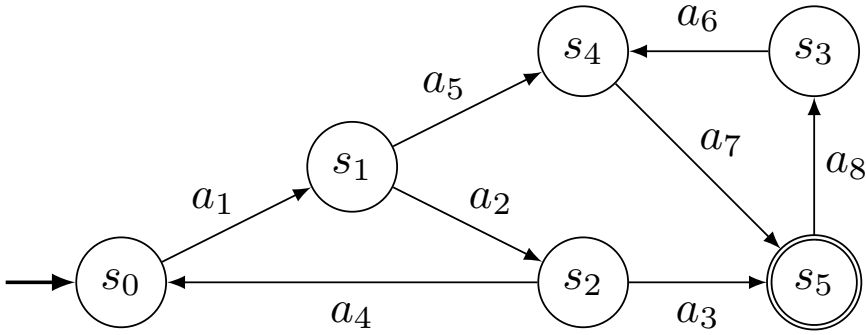
\includegraphics[width=0.7\linewidth]{assets/img_4_3.jpg}
    % \caption{State space}
    % \label{fig:layout}
\end{figure}\\
We define a heuristic $h$ as follows:
$h = \{ s_0 \mapsto 3, s_1 \mapsto 2, s_2 \mapsto 1, s_3 \mapsto \infty,
s_4 \mapsto \infty, s_5 \mapsto \infty \}$
\begin{itemize}
    \item $h$ is not safe: $h^*(s_4) = 1 \not= h(s_4)$
    \item $h$ is consistent. We will show that $h(s) \leq
    \underbrace{\text{cost}(a)}_{=1} + h(s') = 1 + h(s')$
    for all transitions $s \xrightarrow{a} s'$:
    \begin{itemize}
        \item $s_0 \xrightarrow{a_1} s_1$:
        $h(s_0) = 3 \color{green}\leq \color{black} 3 = 1 + h(s_1)$
        \item $s_1 \xrightarrow{a_2} s_2$:
        $h(s_1) = 2 \color{green}\leq \color{black} 2 = 1 + h(s_2)$
        \item $s_2 \xrightarrow{a_3} s_5$:
        $h(s_2) = 1 \color{green}\leq \color{black} \infty = 1 + h(s_5)$
        \item $s_2 \xrightarrow{a_4} s_0$:
        $h(s_2) = 1 \color{green}\leq \color{black} 4 = 1 + h(s_0)$
        \item $s_1 \xrightarrow{a_5} s_4$:
        $h(s_1) = 2 \color{green}\leq \color{black} \infty = 1 + h(s_4)$
        \item $s_3 \xrightarrow{a_6} s_4$:
        $h(s_3) = \infty \color{green}\leq \color{black} \infty = 1 + h(s_4)$
        \item $s_4 \xrightarrow{a_7} s_5$:
        $h(s_4) = \infty \color{green}\leq \color{black} \infty = 1 + h(s_5)$
        \item $s_5 \xrightarrow{a_8} s_3$:
        $h(s_5) = \infty \color{green}\leq \color{black} \infty = 1 + h(s_3)$
    \end{itemize}
\end{itemize}

\section*{Statement on scientific integrity}
Google Translate was used to assist in translating individual words from
German to English when writing down the exercise solutions.\\
Apart from that, we solved the entire exercise sheet on our own.

\end{document}
